\documentclass[border=2mm]{standalone}
\usepackage{pgfplots,tikz}
\usetikzlibrary{lindenmayersystems}
\pgfplotsset{compat=1.16}
\begin{document}
\begin{tabular}{c c}
\begin{tabular}{l}
\vspace*{-0.5cm}
\begin{tikzpicture}

\draw [l-system={rule set={F -> FF + F + F + FF + F + F - F }, step=27mm, angle=90,
    axiom=F, order=0}] lindenmayer system -- cycle;

\node[right] (a) at (-0.15,-.25) {\small $n = 0$};   
\end{tikzpicture}
\end{tabular}

&
\begin{tabular}{l}
\begin{tikzpicture}
\draw [l-system={rule set={F -> FF + F + F + FF + F + F - F }, step=9mm, angle=90,
    axiom=F, order=1}] lindenmayer system -- cycle;

\node[right] (a) at (-0.15,-.25) {\small $n = 1$};      
\end{tikzpicture}
\end{tabular}

\vspace*{0.75cm}
\\
\begin{tabular}{l}
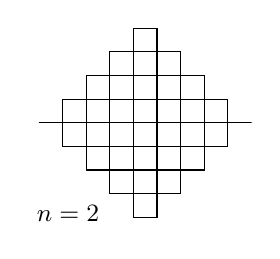
\begin{tikzpicture}
\draw [l-system={rule set={F -> FF + F + F + FF + F + F - F }, step=3mm, angle=90,
    axiom=F, order=2}] lindenmayer system -- cycle;
\node[right] (a) at (-0.15,-1.15) {\small $n = 2$}; 
\end{tikzpicture}
\end{tabular}
&
\begin{tabular}{l}
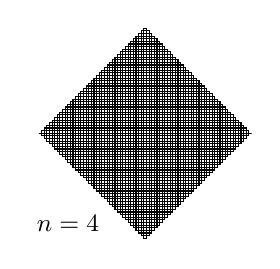
\begin{tikzpicture}
\draw [l-system={rule set={F -> FF + F + F + FF + F + F - F }, step=0.333333mm, angle=90,
    axiom=F, order=4}] lindenmayer system -- cycle;
\node[right] (a) at (-0.15,-1.15) {\small $n = 4$}; 
\end{tikzpicture}
\end{tabular}
\end{tabular}
\end{document}